\documentclass[border=10pt]{standalone}

\usepackage{tikz}
\usepackage{tikzsymbols}
\usetikzlibrary{calc,patterns,shapes.geometric}

\def\centerarc[#1](#2)(#3:#4:#5){\draw[#1] ($(#2)+({#5*cos(#3)},{#5*sin(#3)})$) arc (#3:#4:#5);}

\begin{document}
	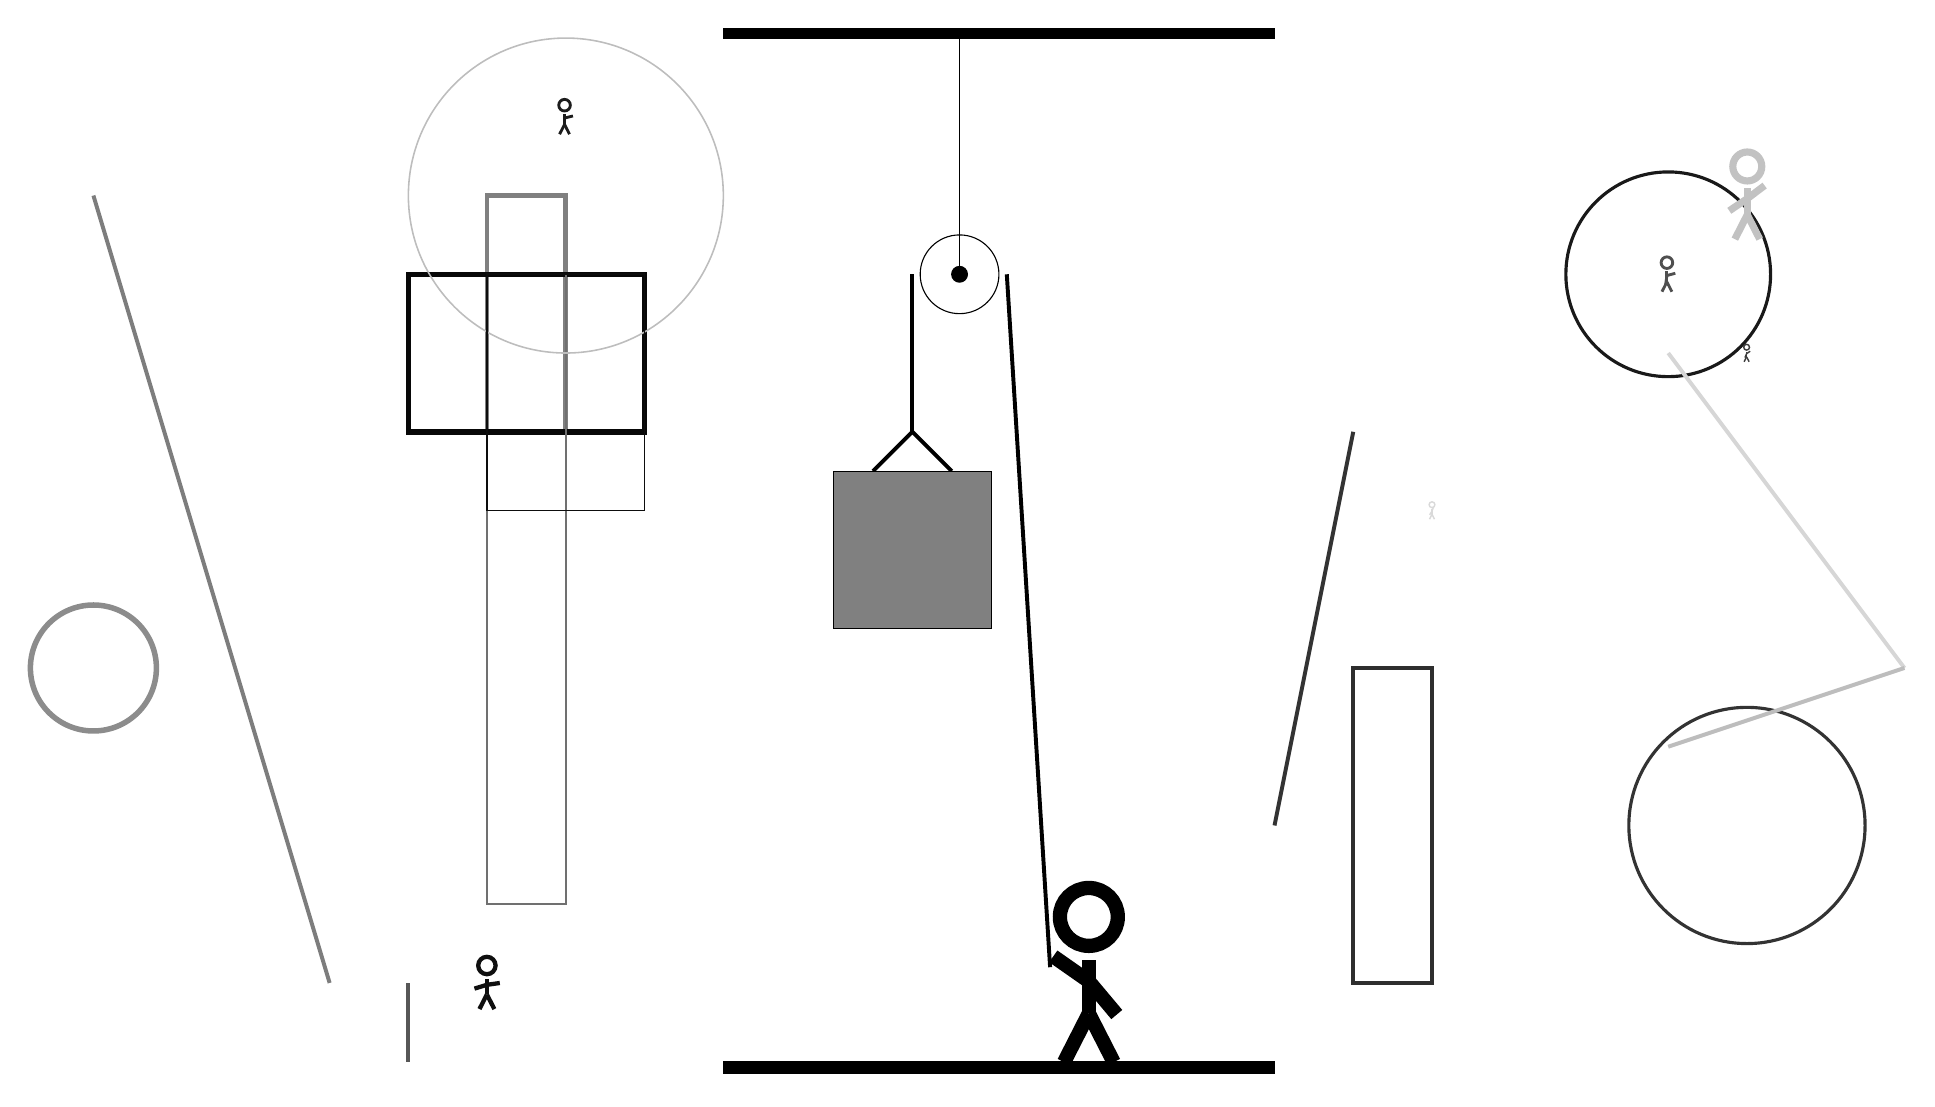
\begin{tikzpicture}
		%%%%% START %%%%%
		
		\draw[fill=black] (-2, 10) rectangle (5, 10.125);
		
		\draw (1, 7) circle (0.5);
		\draw[fill=black] (1, 7) circle (0.1);
		\draw (1, 10) -- (1, 7);
		
		\node[line width=0.7mm, color=black!94] at (-5, -2) {\Strichmaxerl[3][17][8]};
		
		\draw[line width=0.5mm, color=black!51](-7, -2) -- (-10, 8);
		\draw [line width=0.4mm, color=black!90](10, 7) circle (1.3);
		\node[line width=0.7mm, color=black!76] at (11, 6) {\Strichmaxerl[1][67][34]};
		\draw[line width=0.6mm, color=black!50] (-4, 5) rectangle (-5, 8);
		\draw[line width=0.5mm, color=black!80](6, 5) -- (5, 0);
		\draw[line width=0.7mm, color=black!97] (-3, 5) rectangle (-6, 7);
		\draw[line width=0.5mm, color=black!82] (6, 2) rectangle (7, -2);
		\draw [line width=0.4mm, color=black!80](11, 0) circle (1.5);
		\node[line width=0.3mm, color=black!24] at (11, 8) {\Strichmaxerl[5][34][37]};
		\node[line width=0.6mm, color=black!89] at (-4, 9) {\Strichmaxerl[2][90][14]};
		\draw[line width=0.2mm, color=black!56] (-4, -1) rectangle (-5, 7);
		\draw[line width=0.5mm, color=black!16](10, 6) -- (13, 2);
		
		\draw [line width=0.2mm, color=black!26](-4, 8) circle (2.0);
		\draw [line width=0.7mm, color=black!45](-10, 2) circle (0.8);
		\node[line width=0.6mm, color=black!69] at (10, 7) {\Strichmaxerl[2][82][15]};
		\draw[line width=0.5mm, color=black!66](-6, -3) -- (-6, -2);
		\draw[line width=0.5mm, color=black!26](10, 1) -- (13, 2);
		\draw[line width=0.2mm, color=black!95] (-3, 4) rectangle (-5, 7);
		\node[line width=0.5mm, color=black!15] at (7, 4) {\Strichmaxerl[1][57][70]};
		
		\draw[line width=0.5mm] (-0.1, 4.5) -- (0.4, 5.0) -- (0.9, 4.5);
		\draw[fill=black!50] (-0.6, 4.5) rectangle (1.4, 2.5);
		
		\draw[line width=0.5mm] (0.4, 7) -- (0.4, 5.0);
		\centerarc[line width=0.5mm](1, 7)(0:180:0.6);
		\draw[line width=0.5mm](1.6, 7) -- (2.15, -1.8);
		
		\node at (2.6, -1.9) {\Strichmaxerl[10][-35][-50]};
		
		\draw[fill=black] (-2, -3) rectangle (5, -3.15);
		
		%%%%% END %%%%%
	\end{tikzpicture}
\end{document}